\section{Versuchsaufbau und Durchf"uhrung} % (fold)
\label{sec:durchf_uhrung}

\subsection{Versuchsaufbau} % (fold)
\label{sub:aufbau}

\begin{figure}[!h]
	\centering
	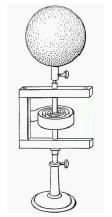
\includegraphics[width = 2cm]{img/Drillachse.PNG}
	\caption{Drillachse mit eingespannter Kugel. \cite{anleitung}}
	\label{drillachse}
\end{figure}

Bei dem Versuch zur Bestimmung des Tr"agheitsmoments $I$ von verschiedenen K"orpern wird eine Drillachse verwendet \ref{drillachse}. Diese besteht aus einer zweifach im Raum drehbar gelagerten Achse, welche "uber eine Spiralfeder mit dem Rahmen verbunden ist.
Auf diese Achse k"onnen die verschiedenen K"orper befestigt werden.

\subsection{Durchf"uhrung} % (fold)
\label{sub:durchf_uhrung}

\subsubsection{Statische Methode} % (fold)
\label{sub:statische_methode}

Ein Metallstab wird symmetrisch und horizontal auf die Drillachse geschraubt. 
Mithilfe einer Federwaage wird die r"ucktreibende Kraft gemessen, die bei dem Auslenkwinkel $\varphi$ wirkt.
Dabei muss die Federwaage senkrecht zum Radius der vom K"orper beschriebenen Kreisbahn gehalten werden.

Diese Messung wird f"ur 10 verschiedene Auslenkwinkel durchgef"uhrt.
Dabei bleibt der Abstand $r$ konstant.

\subsubsection{Dynamische Methode} % (fold)
\label{sub:dynamische_methode}

Eine Metallstange wird horizontal und symmetrisch aud die Drillachse geschraubt.
In einem Abstand $r$ werden symmetrisch Gewichte aufgeschraubt.
Das System wird um einen Winkel $\varphi$ ausgelenkt.
Nach loslassen des Stange schwingt das System und die Schwingungsdauer $3T$ wird gemessen und gemittelt.

Die Schwingungsdauer wird dabei von zwei Uhren gleichzeitig gestoppt.
Diese Messung wird f"ur 10 verschiedene Abst"ande $r$ der Massen zur Drehachse wiederholt.

\subsection{Messung des Tr"agheitsmoments eines K"orpers} % (fold)
\label{sub:tr_agheitsmoment_verschiedener_k_orper}

Auf die Drillachse wird ein K"orper geschraubt.
Die Schwingungsdauer $3T$ wird gemessen und gemittelt.
Diese Messung wird 5 mal wiederholt f"ur eine gro"se Holzkugel und einen Messingzylinder.

\subsection{Messung des Tr"agheitsmoments einer Puppe} % (fold)
\label{sub:messung_des_tr_agheitsmoments_einer_puppe}

Eine Holzpuppe wird auf die Drillachse geschraubt.
Es wird 5 mal die Schwingungsdauer $3T$ gemessen und gemittelt.
Dies wird f"ur insgesamt zwei K"orperhaltungen wiederholt.
Dabei sind einmal die Arme an den K"orper der Puppe angelehnt und einme horizontal seitlich ausgestreckt.
Um die Arme, Beine, der Kopf und der Oberk"orper als Zylinder n"ahern zu k"onnen, werden deren Durchmesser an 10 verschiedenen Stellen gemessen und gemittelt.
Durch die N"aherung kann ein Theoriewert der Puppe errechnet werden.